\documentclass[11pt]{article}
\usepackage[top=1in, bottom=1in, left=1in, right=1in]{geometry}
\usepackage{float}
\usepackage{color}
\usepackage{picture}
\usepackage{listings}
\usepackage{verbatim}
\usepackage{caption}
\usepackage{makeidx}
\usepackage{graphicx}
\usepackage{amsmath}
\usepackage{subcaption}
\usepackage[utf8]{inputenc}
\usepackage[linktocpage=true]{hyperref}
\usepackage{multirow}
\usepackage{rotating}
\usepackage{lscape}
\makeatletter
\newcommand{\rmnum}[1]{\romannumeral #1}
\newcommand{\Rmnum}[1]{\expandafter\@slowromancap\romannumeral #1@}
\makeatother

% Used for the figures that have been inserted into the document.
\floatstyle{plain} 
\restylefloat{figure}

% Used so as not to indent paragraphs.
\setlength\parindent{0pt}

% Used for syntax highlighting in code.
\definecolor{skyblue}{rgb}{0.53, 0.81, 0.92}
\definecolor{lightred}{rgb}{0.90, 0.36, 0.36}
\definecolor{darkkhaki}{rgb}{0.71, 0.51, 0.06}

% Default parameters for listings package.
\lstset {
	tabsize=4,
	keywordstyle=\color{darkkhaki},
	commentstyle=\color{blue},
	showstringspaces=false,
	stringstyle=\color{lightred},
	frame=TLRB,
	captionpos=b,
	basicstyle=\small\ttfamily,
	breaklines=true
}

% Default parameters for hyperref package.
\hypersetup {
	pdftoolbar=true,
	pdfmenubar=true,
	colorlinks=true,
	linkcolor=red,
	citecolor=green,
	filecolor=magenta,
	urlcolor=cyan
}

\newcommand{\superscript}[1]{\ensuremath{^{\textrm{#1}}}}
\newcommand{\subscript}[1]{\ensuremath{_{\textrm{#1}}}}

\numberwithin{equation}{section}
%\setcounter{secnumdepth}{0}
\begin{document}

\begin{titlepage}

\begin{center}

\textsc{\LARGE Networks Assignment-4}\\[2.5cm]

\linethickness{0.5mm}
\line(1, 0){1\linewidth} \\[0.2cm]
{\huge \bfseries Packet Capturing Using Wireshark } \\[0.4cm]
\line(1, 0){1\linewidth} \\[2.5cm]

\begin{minipage}[t]{0.4\textwidth}
	\begin{flushleft} \large
	\emph{Prepared by:} \\[0.3cm]
	Nikhil Agarwal \\
	{\small 11012323} \\[0.2cm]
	Himanshu Upreti \\
	{\small 11012315} \\[0.2cm]
	\end{flushleft}
\end{minipage}
\begin{minipage}[t]{0.4\textwidth}
	\begin{flushright} \large
	\emph{Instructors:} \\[0.3cm]
	Dr. Sukumar Nandi\\[0.2cm]
	T. Venkatesh\\
	\end{flushright}
\end{minipage}

\vfill

% Bottom of the page
{\large \today}

\end{center}

\end{titlepage}

%\pagebreak

\renewcommand\contentsname{{\Huge Contents}\vspace{0.5cm}}
\addtocontents{toc}{~\hfill\textbf{Page}\par}
\cleardoublepage
\phantomsection
\addtocontents{toc}{\linespread{1.5}\selectfont}
\addcontentsline{toc}{section}{Contents}
\setcounter{tocdepth}{8}


\cleardoublepage
\phantomsection
%\addcontentsline{toc}{section}{List of Figures}
\renewcommand\listfigurename{{\Huge List of Figures}\vspace{0.5cm}}
\addtocontents{lof}{\linespread{1.5}\selectfont}
\addtocontents{lof}{~\hfill\textbf{Page}\par}
%\listoffigures

\pagebreak

\section*{PartA: Initials}

\textbf{1. NS-3 ( www.nsnam.org) is a discrete event, packet level network simulator for Internet systems. Download and install NS-3. Create a simple topology of two nodes – Node1 and Node2, separated by a point-to-point link. Setup a UdpClient on Node1 and UdpServer on Node2. Start the client application, and measure end to end throughput while varying the latency of the link. Now add another client application to Node1 and a server instance to Node2. What you need to configure to ensure that there is no conflict? Measure end-to-end throughput with the extra client and server application instances. Show screenshots of pcap traces which indicate that delivery is made to the appropriate server instance. }\\

\textbf{ 2. Make the following simulations in NS-3}\\

\textbf{Make a topology of 4 nodes in the following way.}\\

\begin{figure}[H]
\begin{center}
		\centering
		\resizebox{1\linewidth}{!}{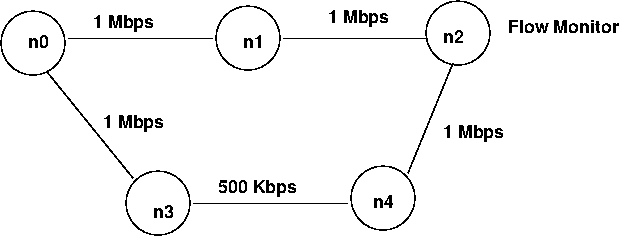
\includegraphics{pic_1}}
		\caption{Topology of four nodes}
		\label{fig:q1_f1_a}
\end{center}
\end{figure}

\textbf{n0 starts CBR traffic at time 1.0 of rate 900 Kbps destined for n2. n0 starts another CBR traffic at time 1.5 of rate 300 Kbps destined for node n1. At time 2.0, link from n0 to n1 goes down. Use a dynamic routing protocol so that path n0-n3-n2 is used now At time 2.7, link n0-n1 comes up again. At time 3.0, CBR traffic destined for node n1 stops. CBR destined for n2 stops at time 3.5. Use a  Flow monitor to monitor losses at n2. Draw a graph of percentage loss as a function of time for the duration of simulation. Give an explanation for results you find. }\\

\textbf{3. Consider following topology}\\


\begin{figure}[H]
\begin{center}
		\centering
		\resizebox{1\linewidth}{!}{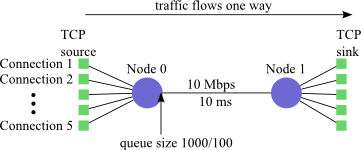
\includegraphics{pic_2}}
		\label{fig:q1_f1_a}
\end{center}
\end{figure}
 
\textbf{Connection 1 starts at time 0, Connection 2 at time 5, Connection 3 at time 10, Connection 4 at time 15, and Connection 5 at time 20. End Connection 1 at time 50.1, Connection 2 at time 45, Connection 3 at time 40, Connection 4 at time 35, and Connection 5 at time 30.}\\

\textbf{Using the generated trace files, produce graphs for the following:}\\

\textbf{a) The receivers' rates over time. Calculate the rate for each TCP connection separately. Plot the rate for all of the receivers on the same graph. To plot a smooth rate, calculate the rate over a moving window of 10 packets. You can do this by plotting a point every time a packet is received. if $packet_i$ is received at time $t_i$, plot a point at $t_i$ equal to the sum of the lengths of $packet_{i-10}$ through $packet_i$, divided by the $t_i$ - $t_{i-10}$. You will need to modify this slightly to handle the start of the connection, when there are fewer than 10 previous packets.}\\

\textbf{b) The queue size over time and each packet drop event. You can calculate the queue size at any time by observing all packet enqueue, dequeue, and drop events. Plot each drop event at the maximum queue size  when the drop occurs using an "X" symbol.}\\

\textbf{c) The Congestion Window over time for each TCP connection.}\\

\textbf{ Use only TCP NewReno for this experiment. Turn in all of your graphs and then answers to the following questions}\\

\textbf{a) What do you observe about fairness among the various TCP connections?}\\
 
\textbf{b) What do you observe about the queue size and packet drops?}\\

\textbf{4. Consider the following topology }\\


\begin{figure}[H]
\begin{center}
		\centering
		\resizebox{1\linewidth}{!}{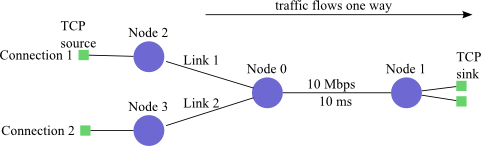
\includegraphics{pic_3}}
		\label{fig:q1_f1_a}
\end{center}
\end{figure}

\textbf{The queue size limit on all nodes is 10. The bandwidth on Links 1 and 2 is 1.5 Mbps. The propagation delay on Links 1 and 2 is initially 10 ms, but you will be varying the propagation delay on Link 2 for your experiments.}\\

\textbf{Connection 1 starts at time 0, using Link 1. Connection 2 starts at time 0. Both connections run for 5 seconds.}\\

\textbf{Plot a graph to show the throughput for each connection over time and observe that they get approximately the same amount. Now run a set of experiments, varying the propagation delay on Link 2 so that Connection 2 has an increasingly longer RTT. Produce the following graph:}\\

\textbf{The receiver's total rate (averaged over the length of the connection) versus the propagation delay on Link 2. Plot each connection separately. }\\

\textbf{Use only TCP NewReno for these experiments. What do you observe about the relationship ? }\\


















\lstinputlisting[caption=\texttt{} HTTP GET/RESPONSE interaction, label=lst:q1_prog1, language=HTML]{partb_1.txt}





















\begin{table}[H]
\begin{center}
    \begin{tabular}{|c|c|c|}
    \hline
    Ack Segment no. & Ack Sequence no. & Acknowledged Data\\ \hline
 
    1 & 493 & 493\\ \hline
    2 & 1953 & 1460  \\ \hline
    3 & 3413 & 1460\\ \hline
    4 & 4873 & 1460\\ \hline
    5 & 6333 & 1460 \\ \hline
    6 & 7793 & 1460\\ \hline
    7 & 7793 & 0\\ \hline  
    8 & 7793 & 0\\ \hline 
    9 & 7793 & 0\\ \hline
    10 & 12173 & 4380\\ \hline 
    11 & 13633 & 1460\\ \hline
    \end{tabular}
\end{center}
\end{table}



\end{document}